\section{Elektrostatik}
 
%\renewcommand{\arraystretch}{2}
\subsection{Wichtige Formeln der Elektrostatik}
  \begin{tabular}[c]{ | p{6.5cm} | p{7cm} | p{4cm} | }
    \hline
    \textbf{Name} & \textbf{Formel} & \textbf{Einheit}\\ 
    \hline
  Dielektrizit�tskonstante
    & $\varepsilon = \varepsilon_r \varepsilon_0 = 
    \varepsilon_r 8.8542 \cdot 10^{-12} $ & $ \frac{As}{Vm}$ \\
    \hline
  Ladung
    & $Q = I t = C U$
    & $[Q] = As = C$ \\
    \hline
  Elementarladung
    & $e = 1.602 \cdot 10^{-19}$
    & C \\
    \hline
  Arbeit = Energie
    & $W_{AB} = \int \limits^b_a F(r) dr \qquad W = \int \limits^{t_1}_{t_2} p(t)
    dt$ 
    & $[W] = Ws = J; [p] = W$ \\
    \hline
  Coulombsches Gesetz (zw. 2 Q) $^{1)}$
    & $\vec{F} = \vec{E}\cdot Q \qquad F = \frac{Q_1 \cdot Q_2}{4 \pi \varepsilon
    r^2}$ & ($F>0 \rightarrow$ Abstossung) \\ \hline
  Elektrische Feldst�rke $^{2)}$
    & $\vec{E} = \frac{Q}{4\pi\varepsilon r^2} \vec{e}_r , E=\frac{Q}{4\pi\varepsilon r^2}$
    & $[E] = \frac{V}{m}$ \\
    \hline
  Potential 
    & $\varphi = \frac{W}{Q}$
    & \multirow{5}{*}{$[\varphi] = V = \frac{Ws}{As} = \frac{VAs}{As}$}
    \\ & $U_{AB} = \varphi_A - \varphi_B$ 
    & \\
    \cline{1-2}
  Potential einer Pt.-Q. 
    & $\varphi = \frac{Q_1}{4 \pi \varepsilon r}$ 
    & \\
    \cline{1-2}
  �berlagerung $>1$ Pt.-Q. $^{3)}$
    & $\varphi = \frac{1}{4 \pi \varepsilon} \sum\limits_{i=1}^n \frac{Q_i}{r_i}$
    & \\
    \cline{1-2}
  Spannung innerh. E-Feld $^{4)}$
    & $U_{AB} = \int\limits_A^B \vec{E}(s) d\vec{s}$
    & \\
    \hline
  Arbeit im homogenen E-Feld $^{5)}$
    & $W_{AB} = U_{AB} \cdot Q = E \cdot s_{AB} \cdot Q \cdot \cos(\alpha) $
    & $[W] = Ws = J; [p] = W$\\
    \hline
  Elektrische Flussdichte $^{6)}$
    & $\vec{D} = \varepsilon \cdot  \vec{E} = \frac{\Psi}{A} \vec{e}_r =
    \frac{Q}{A} $ & $[D] = \frac{C}{m^2} = \frac{As}{m^2}$
    \\
    & $D$ ist materialunabh�ngig 
    & \\
    \hline
  Elektrischer Fluss
    & $\Psi = \int\limits_A \vec{D} \cdot d \vec{A} \text{ od. } D \cdot dA \cdot \cos \phi$
    & $[\Psi] = As, C$ \\
    \hline
  Gauss'scher Satz der Elektrostatik 
    & $ \Psi_{Huelle} = \sum Q_{eingeschlossen} $ 
    & \\
    \hline
  Kapazit�t
    & $C = \frac{Q}{U}$
    & $[C] = F = \frac{C}{V} = \frac{As}{V}$ \\
    \hline
  Fl�chenladungsdichte
    & $\sigma = \frac{Q}{A}$
    & $ [\sigma] = \frac{C}{m^2} $\\
    \hline
  Energiedichte
      & $w=\frac{W}{V} = \frac{1}{2} \varepsilon \cdot E^2 = \frac{1}{2}D\cdot E$
      & $[w]=\frac{J}{m^3}$ \\
      \hline
  \end{tabular}
  \renewcommand{\arraystretch}{1}

\subsection{Anmerkungen zu den Formeln}
  \textbf{1)} Gilt nur f�r Punktladungen exakt; f�r
  geladene K�rper nur wenn K�rperabmessung $\ll$ Abstand \\
  \textbf{2)} $Q > 0$: $\vec{E}$ gleiche Richtung wie $\vec{e}_r$
  $\leftrightarrow$ $Q < 0$: $\vec{E}$ entgegengesetzte Richtung wie $\vec{e}_r$t.
  Der Radius wird immer von der Kugelmitte aus genommen (d.h. an einer
  Kugeloberfl�che besteht eine Feldst�rke!)\\
  \textbf{3)} Weg AB so w�hlen, dass $\vec{E} \perp \vec{s}$ oder $\vec{E}
  \parallel \vec{s}$.\\
  \textbf{5)} Wird eine Ladung von A nach B verschoben, so h�ngt die
  aufzubringende bzw. abgeg. Energie \textit{nicht vom Verschiebungsweg}, sondern
  nur von der Potentialdifferenz $\varphi_B - \varphi_A$ ab (darum
  $\cos(\alpha)$). $\alpha$ ist der Winkel, wo beide Vektoren $\vec{E}, \vec{s}$
  in dieselbe Richtung zeigen.\\
  \textbf{6)} Im Leiter existiert kein Feld $\Rightarrow D = 0$!
  
\subsection{Energie und Kraft im elektrostatischen Feld}
Im Kondensator gespeicherte Energie: $\qquad W = \frac{1}{2} \cdot C \cdot U^2 = \frac{1}{2} \cdot Q \cdot U = \frac{1}{2} \cdot \frac{Q^2}{C}$ \\
\parbox{5cm}{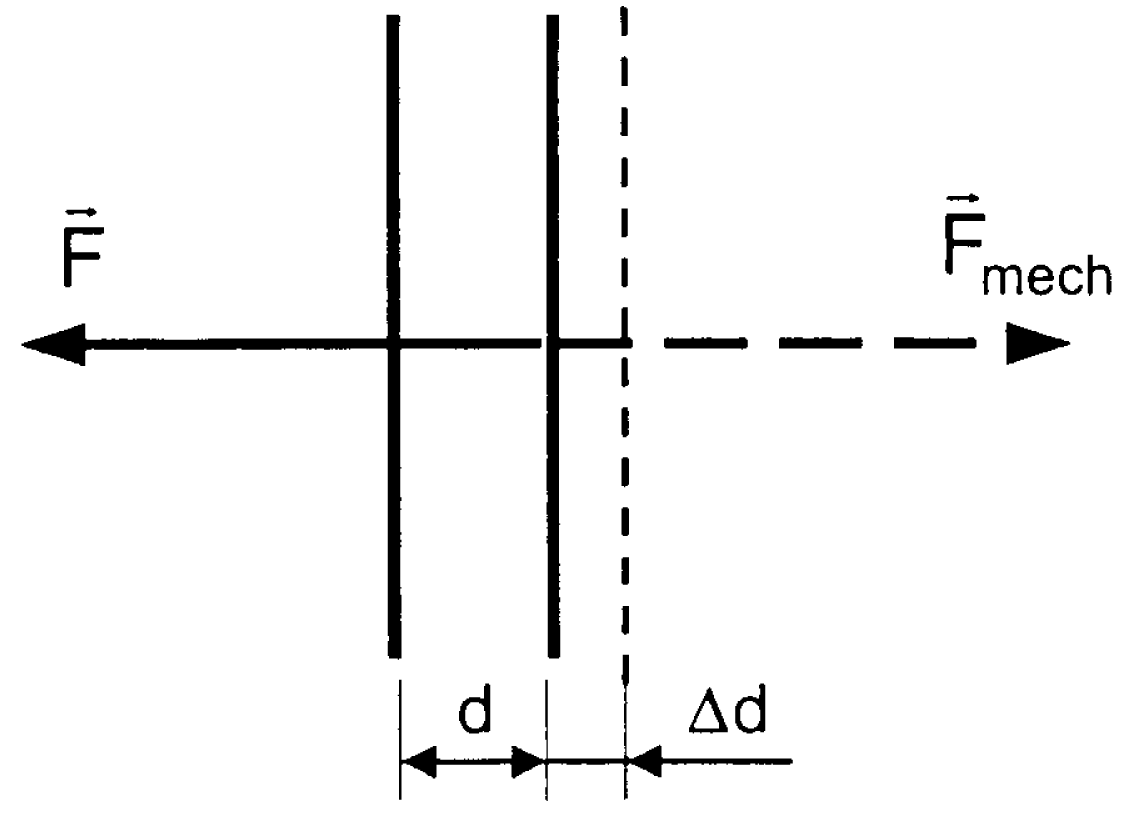
\includegraphics[width=4cm]{./pics/e-c-kraft}}
\parbox{13cm}{
  Grunds�tzlich versuchen sich die Feldlinien zu verk�rzen $\rightarrow$ Die Kraft auf die Grenzfl�chen ist so gerichtet, dass sie die Kapazit�t zu vergr�ssern sucht. \\ 
  Die Kraft berechnet sich mittels dem \textbf{Prinzip der virtuellen Verschiebung}. \\ \\
  $\qquad F = F_{mech} = \left| \frac{\Delta W}{\Delta d} \right| \qquad$ 
  $\Delta W = \frac{1}{2} \varepsilon \cdot E^2 \cdot A \cdot \Delta d \quad
  \Rightarrow \quad F = \frac{1}{2} \varepsilon \cdot E^2 \cdot A = \frac{1}{2} \varepsilon \cdot \frac{U^2}{d^2} \cdot A$ \\
  $ F = \frac{1}{2} \cdot U^2 \cdot \frac{\Delta C}{\Delta d}, \text{ (f�r U =
  const.)} \qquad \text{ oder } \qquad F = \frac{1}{2} \cdot Q^2 \cdot
  \frac{\mathrm d}{\Delta d} \left( \frac{1}{C} \right), \text{ (f�r Q = const.)}$ \\ }
  
  